\begin{pastexam}[label={px:ntu-110-esoe-ds-06}]{臺大工科海洋所 110 學年度（A）第 6 題}
（追蹤）

\textbf{(10 \%)} What does the 2-3-4 tree on the right look like after \textsf{remove(2)}?
\begin{center}
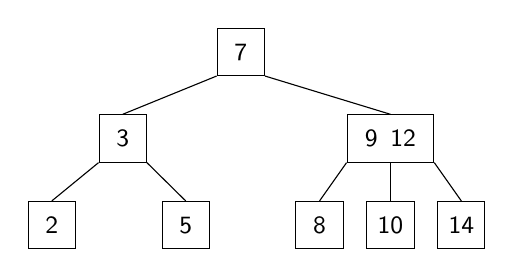
\begin{tikzpicture}[k/.style={rectangle,draw,minimum height=6mm,minimum width=6mm,inner sep=2pt,font=\small\sffamily}]
\node[k] (7) at (0,0) {7};
\node[k] (3) at (-1.5,-1.1) {3}; \node[k,minimum width=11mm] (912) at (1.9,-1.1) {9\enspace 12};
\node[k] (2) at (-2.4,-2.2) {2}; \node[k] (5) at (-0.7,-2.2) {5};
\node[k] (8) at (1.0,-2.2) {8}; \node[k] (10) at (1.9,-2.2) {10}; \node[k] (14) at (2.8,-2.2) {14};
\draw (7.south west) -- (3.north); \draw (7.south east) -- (912.north);
\draw (3.south west) -- (2.north); \draw (3.south east) -- (5.north);
\draw (912.south west) -- (8.north); \draw (912.south) -- (10.north); \draw (912.south east) -- (14.north);
\end{tikzpicture}
\end{center}
\end{pastexam}

\begin{pastsoln}
刪除照資結書第~11.1.4~節的規則（2-3-4 樹和 2-3 樹相同，第~11.1.5~節）：在葉子拿掉鍵；葉子變空
（不足）時，相鄰的兄弟有多的鍵就\textbf{借}（父節點的分隔鍵下來，兄弟的鍵上去），兄弟都只有一個
鍵就\textbf{合併}（空節點、父節點的分隔鍵、兄弟合成一個節點），父節點因此變空就往上用同樣的方法
處理。

\textbf{第 1 步：拿掉 2。} $2$ 在葉子 $[2]$ 裡，拿掉後這片葉子變空。 它唯一相鄰的兄弟 $[5]$ 只有一個鍵，
不能借，只好合併：父節點 $[3]$ 的分隔鍵 $3$ 下來，和 $5$ 合成 $[3\ 5]$。 父節點 $[3]$ 因此變空，只剩一個
子節點 $[3\ 5]$。
\begin{center}
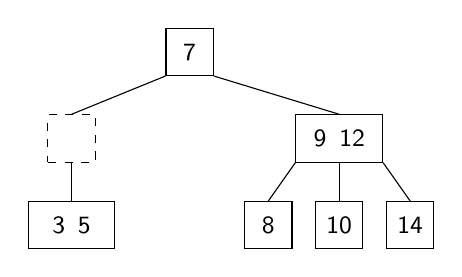
\begin{tikzpicture}[k/.style={rectangle,draw,minimum height=6mm,minimum width=6mm,inner sep=2pt,font=\small\sffamily}]
\node[k] (7) at (0,0) {7};
\node[k,dashed] (e) at (-1.5,-1.1) {\phantom{0}}; \node[k,minimum width=11mm] (912) at (1.9,-1.1) {9\enspace 12};
\node[k,minimum width=11mm] (35) at (-1.5,-2.2) {3\enspace 5};
\node[k] (8) at (1.0,-2.2) {8}; \node[k] (10) at (1.9,-2.2) {10}; \node[k] (14) at (2.8,-2.2) {14};
\draw (7.south west) -- (e.north); \draw (7.south east) -- (912.north);
\draw (e.south) -- (35.north);
\draw (912.south west) -- (8.north); \draw (912.south) -- (10.north); \draw (912.south east) -- (14.north);
\end{tikzpicture}
\end{center}

\textbf{第 2 步：處理變空的內部節點。} 它的兄弟 $[9\ 12]$ 有兩個鍵，可以借：根的分隔鍵 $7$ 下來放進
空的節點，兄弟靠近這一邊的鍵 $9$ 上去取代根的 $7$，兄弟靠近這一邊的子樹 $[8]$ 也跟著搬過來，成為
$7$ 的右子節點。 根仍有一個鍵，結束。
\begin{center}
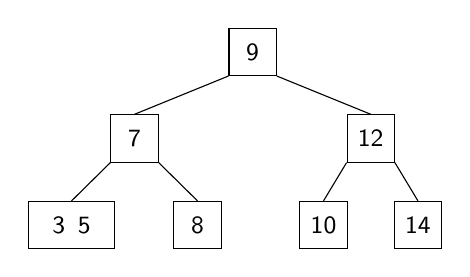
\begin{tikzpicture}[k/.style={rectangle,draw,minimum height=6mm,minimum width=6mm,inner sep=2pt,font=\small\sffamily}]
\node[k] (9) at (0,0) {9};
\node[k] (7) at (-1.5,-1.1) {7}; \node[k] (12) at (1.5,-1.1) {12};
\node[k,minimum width=11mm] (35) at (-2.3,-2.2) {3\enspace 5}; \node[k] (8) at (-0.7,-2.2) {8};
\node[k] (10) at (0.9,-2.2) {10}; \node[k] (14) at (2.1,-2.2) {14};
\draw (9.south west) -- (7.north); \draw (9.south east) -- (12.north);
\draw (7.south west) -- (35.north); \draw (7.south east) -- (8.north);
\draw (12.south west) -- (10.north); \draw (12.south east) -- (14.north);
\end{tikzpicture}
\end{center}
這就是答案：根 $[9]$；左子節點 $[7]$，底下是 $[3\ 5]$ 和 $[8]$；右子節點 $[12]$，底下是 $[10]$ 和 $[14]$。
檢查：中序是 $3, 5, 7, 8, 9, 10, 12, 14$，由小到大；所有葉子都在同一層，每個節點 $1$--$3$ 個鍵。

如果用由上而下的刪除（往下走時先把要進去的 2-節點補成至少 2 個鍵）：在根要走進 $[3]$，兄弟
$[9\ 12]$ 有多的鍵，先借，得到根 $[9]$、左子節點 $[3\ 7]$（子節點 $[2]$、$[5]$、$[8]$）、右子節點
$[12]$；再要走進 $[2]$，兄弟 $[5]$ 只有一個鍵，合併成 $[2\ 3\ 5]$，父節點剩 $[7]$；最後在葉子拿掉 $2$。
結果和上面完全一樣。

常見的錯是第 1 步向不相鄰的 $[9\ 12]$ 借鍵；借只能找相鄰的兄弟，$[2]$ 唯一的兄弟是 $[5]$。
\end{pastsoln}
